\chapter{Сравнение работы метода дифференцируемого рендеринга разреженных SDF}
\label{ch:chap4}

Этот раздел состоит из двух частей: в первой части приводится сравнение с базовым методом по времени реконструкции, качеству и размеру полученных моделей; вторая часть посвящена исследованию вклада отдельных компонентов предложенного метода (абляционному исследованию). Все эксперименты проводились на процессоре AMD Ryzen 9 7950X и графическом процессоре NVIDIA GeForce RTX 4090.

\section{Сравнения.}

Сравнения представляют собой реконструкцию моделей в максимально равных условиях с последующим сопоставлением времени, точности реконструкции, а также размеров полученных представлений для каждой эпохи. Реализация метода релаксированной границы взята из официального репозитория \cite{DRSDF24Repo}.

Реконструкция велась на 24 ракурсах, равномерно распределённых на полусфере, разрешение изображений 1024*1024. В сцене два направленных источника света: (1,1,1) и (-1,-1,-1), а также ambient light. В обоих методах используется одна и та же модель переноса света: прямое освещение ламбертовской поверхности без вторичных лучей (в базовом методе трассировка путей отключена), поэтому различия в скорости и точности определяются представлением и алгоритмами, а не моделью освещения. Размер батча 6. Гиперпараметры, такие как learning rate, параметры оптимизатора Adam, ширина релаксированной границы, взяты из конфигурационного файла в репозитории базового метода. Восстанавливались 12 моделей: 4 модели из Стэнфордского репозитория 3D сканов (Armadillo, Bunny, Dragon, Happy), скан бюста Нефертити (Nefertiti), чайник из Юты (Teapot), а также другие сканы: Buggy, Demogorgon, Doom, Helicopter, Pufferfish, Wheel.

Если не оговорено иное, результаты предложенного метода получены в основном режиме: 7 эпох, с маской объекта и с дополнительным разреживанием в течение эпохи\footnote{Кроме того, после каждого увеличения разрешения сетка разреживалась повторно: при увеличении разрешения каждый брик делится на 8, поэтому слой бриков вокруг поверхности становится вдвое толще. Повторное разреживание сокращает время следующей эпохи вплоть до двух раз, но замедляет рост тонких деталей. Для модели Helicopter оно применялось только перед последней эпохой, иначе одна из лопастей винта не успевала восстановиться.}. Результаты для 5 эпох взяты из того же запуска после окончания пятой эпохи и приводятся только для сравнения с базовым методом при одинаковом числе эпох.

\begin{figure}[t]
    \centering
    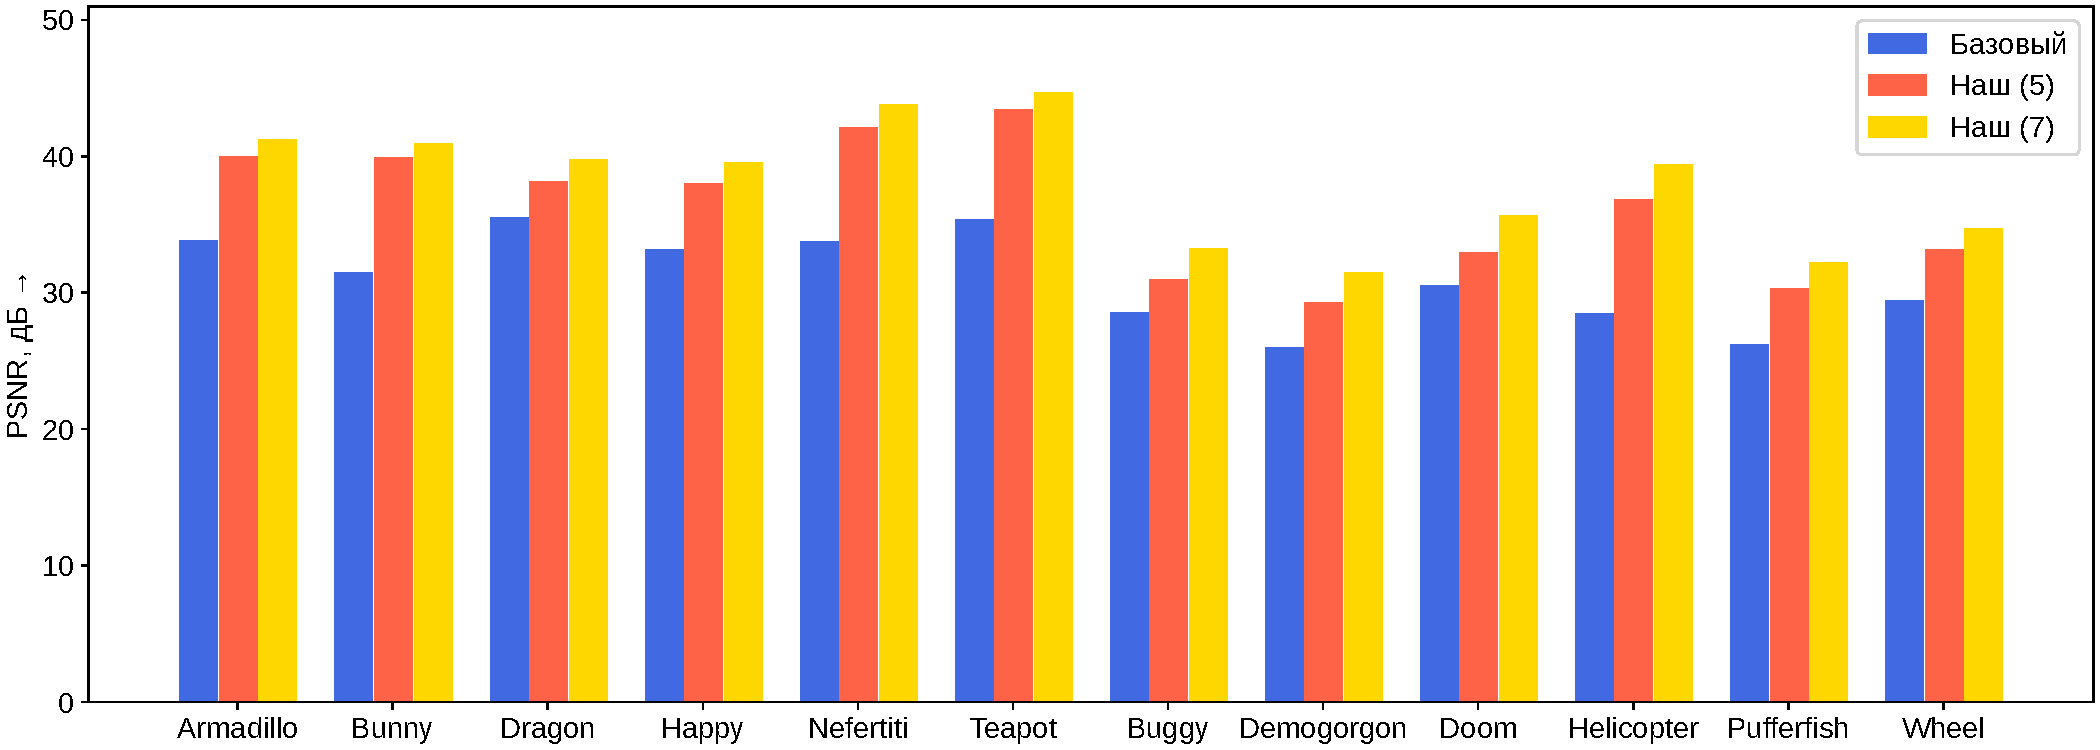
\includegraphics[width=0.99\textwidth]{ieee_acc_psnr_all.pdf}
    \caption{Среднее значение PSNR восстановленных моделей для базового метода, нашего метода с тем же числом эпох (5 эпох), и нашего метода с тем же временем реконструкции (7 эпох).}
    \label{figPSNR57}
\end{figure}

\begin{figure}[h]
    \centering
    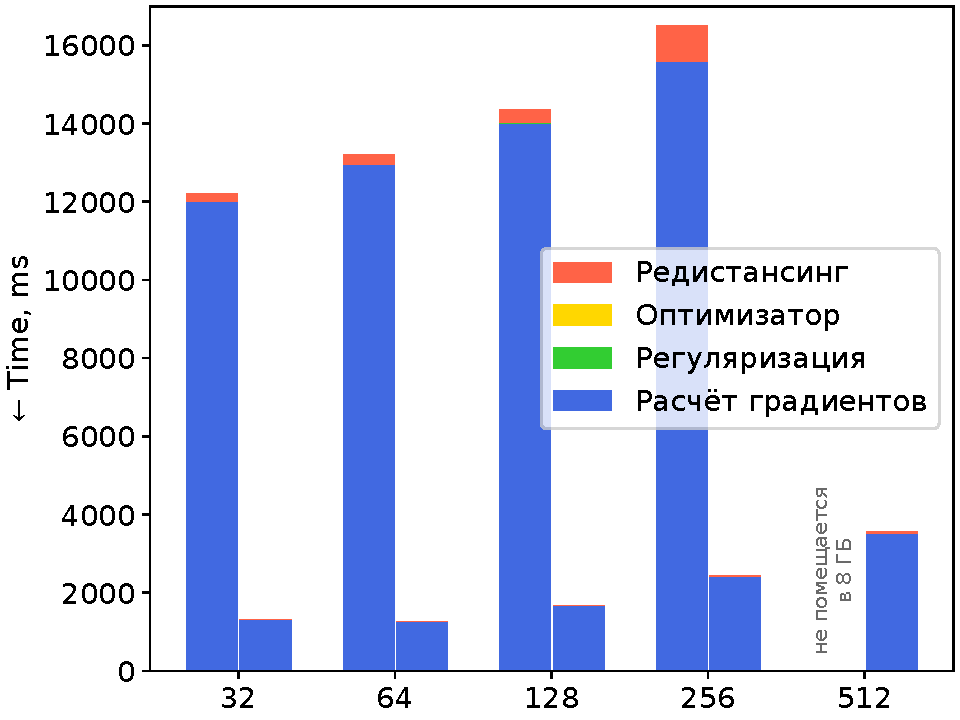
\includegraphics[width=0.7\textwidth]{ieee_acc_time_5.pdf}
    \caption{Среднее время выполнения одной итерации для эпох 1--5.}
    \label{figTime5}
\end{figure}

Базовый метод в нашей аппаратной конфигурации способен выполнить только 5 эпох (после чего Dr.JIT возвращает ошибку "out of memory", то есть данные не умещаются в 24 гигабайта памяти графического процессора), в то время как наш метод выполняет 7 эпох за то же время. Поэтому в сравнении с базовым методом мы демонстрируем время для первых пяти эпох, а качество как для одинакового числа эпох, так и для одинакового времени выполнения.

На Рис. \ref{figTime5} представлено среднее по всем моделям время выполнения одной итерации для первых пяти эпох. По нему видно, что у SBS появляется зависимость времени рендера от размера модели; тем не менее, наш метод превосходит базовый на первых пяти эпохах. Отдельно следует отметить редистансинг: локальная версия на CPU оказалась быстрее, чем dense grid redistancing on GPU.

Рис. \ref{figPSNR57} показывает среднее по ракурсам значение PSNR для рендеров референса и реконструкции. Представлено три результата: работа базового метода (5 эпох), работа нашего метода также для 5 эпох, а также за то же время, которое работал базовый метод (7 эпох). Первые 6 моделей обладают достаточно гладкими поверхностями, поэтому наш метод показывает гораздо лучшую точность реконструкции за счёт более высокой детализации используемого представления. Последние 6 моделей отличаются рельефностью и обилием мелких деталей, и точность их реконструкции ниже у обоих методов: при освещении без вторичных лучей мелкие детали и затенённые полости воспроизводятся хуже. Учёт вторичных лучей может повысить точность на таких моделях. Использование этих моделей в будущих сравнениях позволит нагляднее продемонстрировать прогресс и эффективность метода.

\begin{table}
    \centering
    \begin{tabular}{ccccccc}
        \toprule
        Представление & $128^3$ & $256^3$ & $512^3$ & $1024^3$ & $2048^3$ \\
        \midrule[\heavyrulewidth]
        Базовый метод (плотная сетка) & 8 & 64 & 512 & 4096* & 32768* \\
        \cmidrule(lr){1-6}
        Наш метод (Armadillo) & \textbf{4.0} & \textbf{16.1} & \textbf{65.4} & \textbf{265.5} & \textbf{1065.8} \\
        \cmidrule(lr){1-1} \cmidrule(lr){2-6}
        Наш метод (Bunny) & \textbf{6.0} & \textbf{25.1} & \textbf{101.6} & \textbf{406.9} & \textbf{1611.0} \\
        \cmidrule(lr){1-1} \cmidrule(lr){2-6}
        Наш метод (Dragon) & \textbf{2.2} & \textbf{8.7} & \textbf{35.2} & \textbf{147.6} & \textbf{602.2} \\
        \cmidrule(lr){1-1} \cmidrule(lr){2-6}
        Наш метод (Happy) & \textbf{2.6} & \textbf{11.6} & \textbf{50.3} & \textbf{210.4} & \textbf{846.6} \\
        \cmidrule(lr){1-1} \cmidrule(lr){2-6}
        Наш метод (Nefertiti) & \textbf{3.5} & \textbf{14.6} & \textbf{59.3} & \textbf{238.2} & \textbf{951.0} \\
        \cmidrule(lr){1-1} \cmidrule(lr){2-6}
        Наш метод (Teapot) & \textbf{3.0} & \textbf{12.1} & \textbf{49.2} & \textbf{200.8} & \textbf{802.0} \\
        \cmidrule(lr){1-1} \cmidrule(lr){2-6}
        Наш метод (Buggy) & \textbf{3.9} & \textbf{18.3} & \textbf{85.2} & \textbf{375.8} & \textbf{1494.6} \\
        \cmidrule(lr){1-1} \cmidrule(lr){2-6}
        Наш метод (Demogorgon) & \textbf{5.3} & \textbf{23.4} & \textbf{105.9} & \textbf{459.1} & \textbf{1842.8} \\
        \cmidrule(lr){1-1} \cmidrule(lr){2-6}
        Наш метод (Doom) & \textbf{4.6} & \textbf{20.7} & \textbf{95.6} & \textbf{423.6} & \textbf{1719.5} \\
        \cmidrule(lr){1-1} \cmidrule(lr){2-6}
        Наш метод (Helicopter) & \textbf{3.4} & \textbf{12.0} & \textbf{41.5} & \textbf{150.3} & \textbf{280.3} \\
        \cmidrule(lr){1-1} \cmidrule(lr){2-6}
        Наш метод (Pufferfish) & \textbf{4.3} & \textbf{23.2} & \textbf{101.4} & \textbf{371.0} & \textbf{1381.5} \\
        \cmidrule(lr){1-1} \cmidrule(lr){2-6}
        Наш метод (Wheel) & \textbf{3.8} & \textbf{18.6} & \textbf{82.1} & \textbf{334.1} & \textbf{1303.5} \\
        \bottomrule
    \end{tabular}
    \caption{Размер моделей для методов Relaxed Boundary и SparseDR на эпохах 3--7. Все значения приведены в мегабайтах. Звёздочками отмечены теоретические значения, поскольку мы не смогли получить их на использовавшемся оборудовании (OOM в Dr. JIT). Для базового метода указан размер сетки, а для нашего метода — суммарный размер SBS и его BVH. Таблица характеризует размер геометрического представления, а не полное потребление памяти в процессе реконструкции (см. Таблицу~\ref{tab:comp_mem}).}
    \label{tab:comp_size}
\end{table}

В Таблице \ref{tab:comp_size} приведены размеры моделей, полученных для каждой модели на эпохах 3-7. Размер SDF сетки на каждой эпохе одинаков для всех моделей, поэтому они указаны один раз в верхней строке. В базовом методе в результате апсемплинга размер плотной сетки увеличивается в 8 раз от эпохи к эпохе. Благодаря использованию разреженной структуры данных, размер всех моделей, полученных нашим методом, меньше размера грида, начиная с третьей эпохи. Размер модели в нашем методе после апсемплинга в среднем приблизительно в 4 раза больше исходного (от 1,9 до 5,4 раза в зависимости от модели и эпохи), так как модель хранит только дистанции у поверхности. Таким образом, множитель роста размера за эпоху у нашего метода примерно вдвое меньше, чем у базового. За счёт накопления этой разницы от эпохи к эпохе отношение размеров на конкретном разрешении растёт: на разрешении $512^3$ представление нашего метода меньше плотной сетки в 4,8--15 раз, на $1024^3$ -- в 8,9--28 раз, на $2048^3$ -- в 18--117 раз.


Размер геометрического представления не равен памяти, необходимой для реконструкции: помимо сетки, в процессе оптимизации хранятся градиенты, состояния оптимизатора Adam, изображения батча и референсов, временные буферы рендеринга и рабочие данные редистансинга, а также кэши используемых систем. Поэтому отдельно была измерена пиковая потребляемая память (Таблица~\ref{tab:comp_mem}). Память графического процессора замерялась утилитой \texttt{nvidia-smi} с периодом 0,2~с как общий объём занятой видеопамяти устройства; в него входит около 0,7~ГиБ, занятых до запуска реконструкции другими процессами, а также память, удерживаемая кэширующим аллокатором Dr.Jit. Пиковая память центрального процессора определялась как максимальный размер резидентной памяти процесса (\texttt{/usr/bin/time -v}). Условия совпадают с описанными выше: 24 ракурса $1024\times1024$, батч из 6 изображений, 64 семпла на пиксель, освещение без вторичных лучей. Для базового метода приведены значения для модели Buggy: размеры плотной сетки и всех рабочих буферов определяются разрешением сетки и изображений, числом семплов и размером батча и не зависят от реконструируемой модели.

\begin{table}[ht]
    \centering
    \small
    \setlength{\tabcolsep}{4pt}
    \begin{tabular}{lcccc}
        \toprule
        Эпоха (сетка) & \multicolumn{2}{c}{Базовый метод} & \multicolumn{2}{c}{Наш метод} \\
        \cmidrule(lr){2-3} \cmidrule(lr){4-5}
         & Сетка, МБ & Пик GPU, ГиБ & Модель, МБ & Пик GPU, ГиБ \\
        \midrule
        1--3 ($32^3$--$128^3$) & 0,1--8 & 3,5 & --- & --- \\
        4 ($256^3$) & 64 & 4,4 & 9--25 & --- \\
        5 ($512^3$) & 512 & 10,4 & 35--106 & --- \\
        6 ($1024^3$) & 4096 & OOM & 148--459 & --- \\
        7 ($2048^3$) & 32768 & OOM & 280--1843 & --- \\
        \midrule
        Пик CPU (весь запуск), ГиБ & \multicolumn{2}{c}{9,9} & \multicolumn{2}{c}{---} \\
        \bottomrule
    \end{tabular}
    \caption{Пиковое потребление памяти в процессе реконструкции. Размеры представлений взяты из Таблицы~\ref{tab:comp_size} (для нашего метода -- диапазон по 12 моделям). OOM -- реконструкция не выполняется на графическом процессоре с 24~ГБ памяти.}
    \label{tab:comp_mem}
\end{table}
% TODO: пиковая память GPU/CPU для SparseDR (те же условия, nvidia-smi + /usr/bin/time -v)

При переходе от $256^3$ к $512^3$ размер плотной сетки увеличивается на 448~МБ, а пиковая видеопамять базового метода -- приблизительно на 6~ГиБ, то есть затраты памяти на рабочие данные, пропорциональные размеру сетки, многократно превышают размер самой сетки. Это объясняет нехватку 24~ГБ видеопамяти базовому методу на следующей эпохе, когда размер сетки (4~ГБ) ещё сам по себе не превышает объём памяти устройства.

\section{Абляционное исследование.}

\begin{figure}[b]
    \centering
    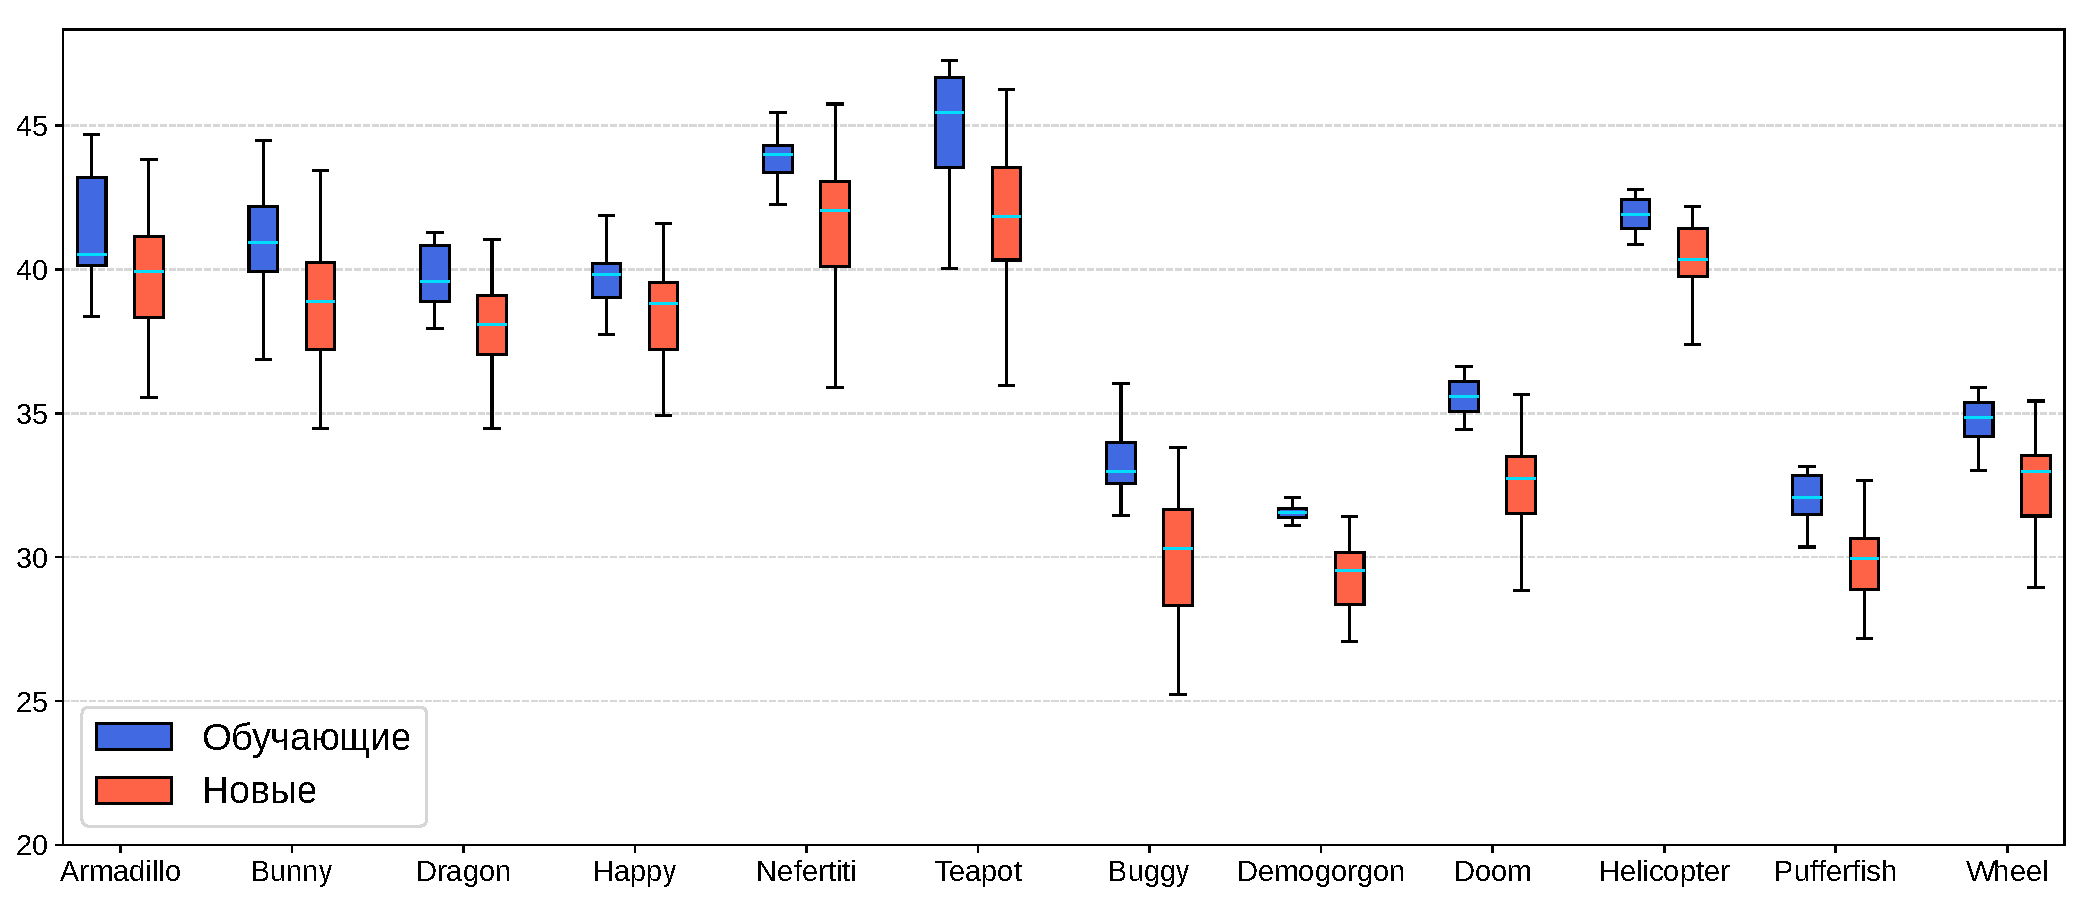
\includegraphics[width=0.99\textwidth]{ieee_acc_psnr_box_nvs.pdf}
    \caption{Усреднённая метрика PSNR на обучающих и новых ракурсах.\label{figNVS}}
\end{figure}

В данном подразделе исследуется влияние отдельных элементов алгоритма и параметров на скорость и качество реконструкции, а также приводятся дополнительные результаты экспериментов из прошлого подраздела, выходящие за рамки сравнения с базовым методом.

% 1. Качество реконструкции на новых ракурсах: Рис. \label{figNVS} показывает значения PSNR для моделей датасета на обучающих и новых ракурсах. Новые ракурсы генерируются на полусфере вокруг объекта, не пересекаясь с обучающими ракурсами. На новых ракурсах качество немного хуже, чем на обучающих, что ожидаемо. При этом среднее различие между PSNR не превышает 3 дБ.

На Рис. \ref{figNVS} приведены значения PSNR, рассчитанные для моделей датасета при рендеринге на обучающих и новых ракурсах. Новые ракурсы генерировались путём равномерной выборки положений камеры на полусфере вокруг объекта, при этом они не совпадали с ракурсами, использованными на этапе обучения. Это позволяет оценить не только точность воспроизведения известных наблюдений, но и способность метода обобщаться на ранее не встречавшиеся положения камеры, что является ключевым аспектом задачи синтеза новых ракурсов (novel view synthesis). Для всех рассмотренных моделей значения PSNR на новых ракурсах несколько ниже, чем на обучающих, что соответствует ожидаемому снижению качества при переходе от известных положений камеры к новым. При этом разница остаётся относительно небольшой, её среднее значение не превышает 3 дБ. Это указывает на отсутствие существенной деградации качества при синтезе новых ракурсов и свидетельствует о способности метода сохранять согласованное представление сцены за пределами обучающей выборки ракурсов.

% 2. Скорость реконструкции с sphere tracing vs. Newton/Analytic
% На Рис. \ref{figSTNt} приведено сравнение времени выполнения эпох с использованием в качестве метода поиска пересечения луча и SBS двух методов: трассировки сферами и метода Ньютона. Из-за необходимости обхода BVH метод трассировки сферами также показывает зависимость от размера модели. Метод Ньютона показывает лучшее время в сравнении с трассировкой сферами на семи эпохах, хотя на 8 эпохе и далее возможно преобладание последнего в связи с дальнейшим увеличением числа вокселей, которые придётся пересекать с лучами.

На рис. \ref{figSTNt} приведено сравнение времени этапа рендеринга на каждой из семи эпох при использовании двух методов поиска пересечений луча с SBS: трассировки сферами и метода Ньютона. Этап рендеринга включает отрисовку батча и накопление градиентов; остальные этапы итерации (регуляризация, шаг оптимизатора, редистансинг) от метода поиска пересечений не зависят и поэтому не показаны. Время работы метода трассировки сферами зависит не только от количества итераций, но и от сложности геометрии модели, поскольку поиск пересечения требует обхода BVH. С увеличением размера модели возрастает число узлов, которые необходимо обойти, что приводит к дополнительным вычислительным затратам.

\begin{figure}[t]
    \centering
    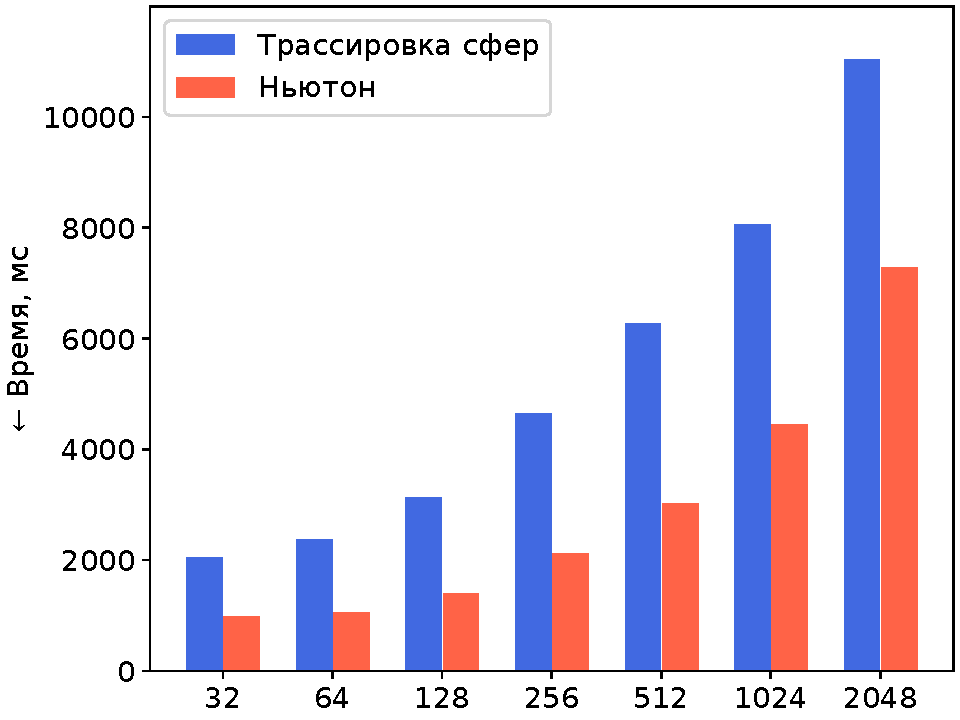
\includegraphics[width=0.7\textwidth]{ieee_acc_time_st_nt.pdf}
    \caption{Среднее по моделям время этапа рендеринга (отрисовка батча с накоплением градиентов) в расчёте на одну итерацию для каждой эпохи: трассировка сферами и метод Ньютона.}
    \label{figSTNt}
\end{figure}

Метод Ньютона демонстрирует меньшее время выполнения по сравнению с трассировкой сферами на первых семи эпохах. Это связано с тем, что при данных размерах SBS число вокселей, пересекаемых лучами, ещё относительно невелико, поэтому итерационный поиск пересечения выполняется быстрее, чем трассировка сферами. Начиная с восьмой эпохи преимущество метода Ньютона может сокращаться или исчезать. При дальнейшем увеличении числа вокселей возрастает количество участков SBS, с которыми требуется вычислить пересечение луча, что увеличивает суммарные затраты на выполнение итераций.

% .3
Ещё один вопрос, требующий рассмотрения -- разница в точности реконструкции при использовании локального редистансинга вместо глобального. На Рис. \ref{figPSNRRedist} приведены сравнения PSNR для реконструкции обоими способами, из которых следует, что различия в точности реконструкции несущественны. Учитывая, что на CPU скорость работы локального редистансинга в среднем в 25-30 раз быстрее, чем глобального, он предпочтителен в использовании в течение эпохи.

\begin{figure}[t]
    \centering
    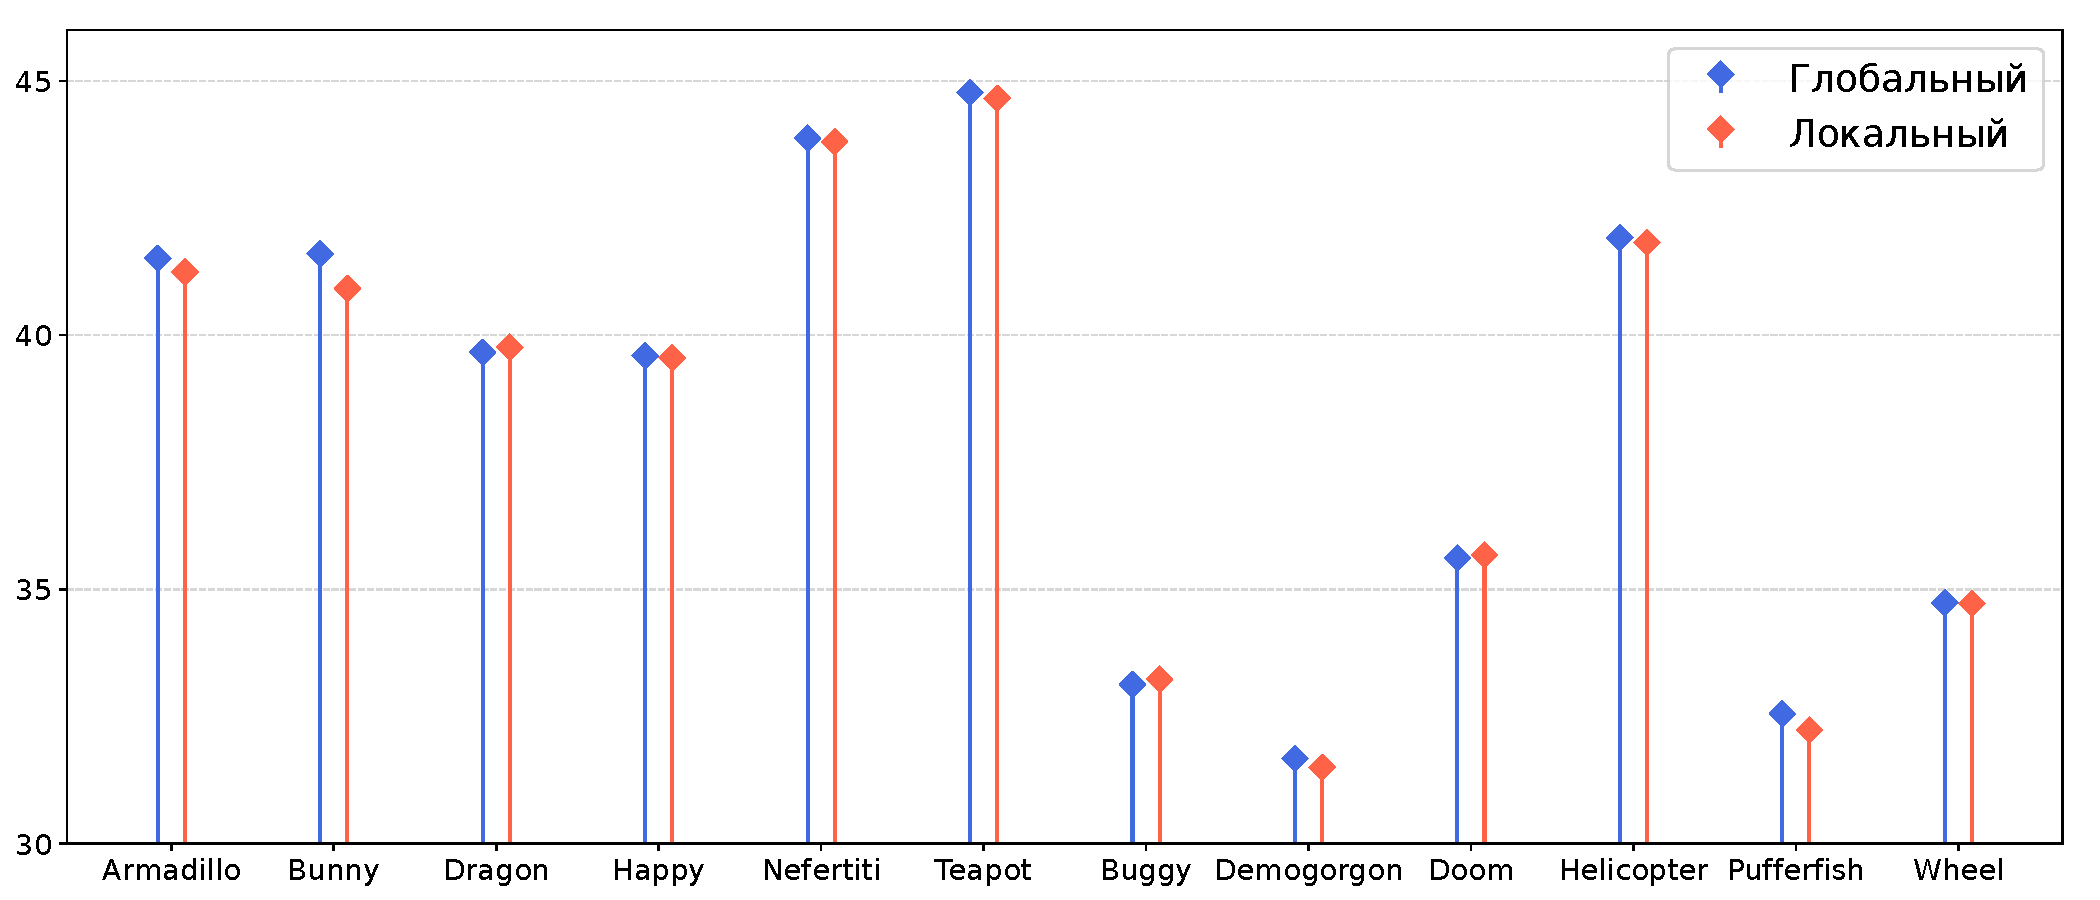
\includegraphics[width=0.9\textwidth]{ieee_acc_psnr_stem_redist.pdf}
    \caption{Среднее значение PSNR для реконструкций с использованием глобального и локального редистансинга на каждой итерации. Глобальный редистансинг по-прежнему дополнительно выполняется между эпохами.}
    \label{figPSNRRedist}
\end{figure}

% 4. Использование маски (параметр чувствительности) -- помогает с отверстиями, приводит к ухудшению качества при злоупотреблении -> Buddha (примеры реконструкции с/без).
В процессе реконструкции можно пользоваться дополнительными инструментами, которые помогут улучшить точность реконструкции моделей. Во-первых, можно использовать маску объекта для референсных изображений. Чувствительность к маске задаётся для каждой эпохи, по умолчанию она равна 0. Повышение её значения может дополнительно помочь с получением отверстий в сложной модели, если непосредственно дифференцируемому рендерингу не удаётся с ними справиться. На Рис. \ref{figAblMask} показаны примеры реконструкции модели Happy Buddha без маски и с ней, а также референсное изображение для наглядности.

\begin{figure}[t]
    \centering
    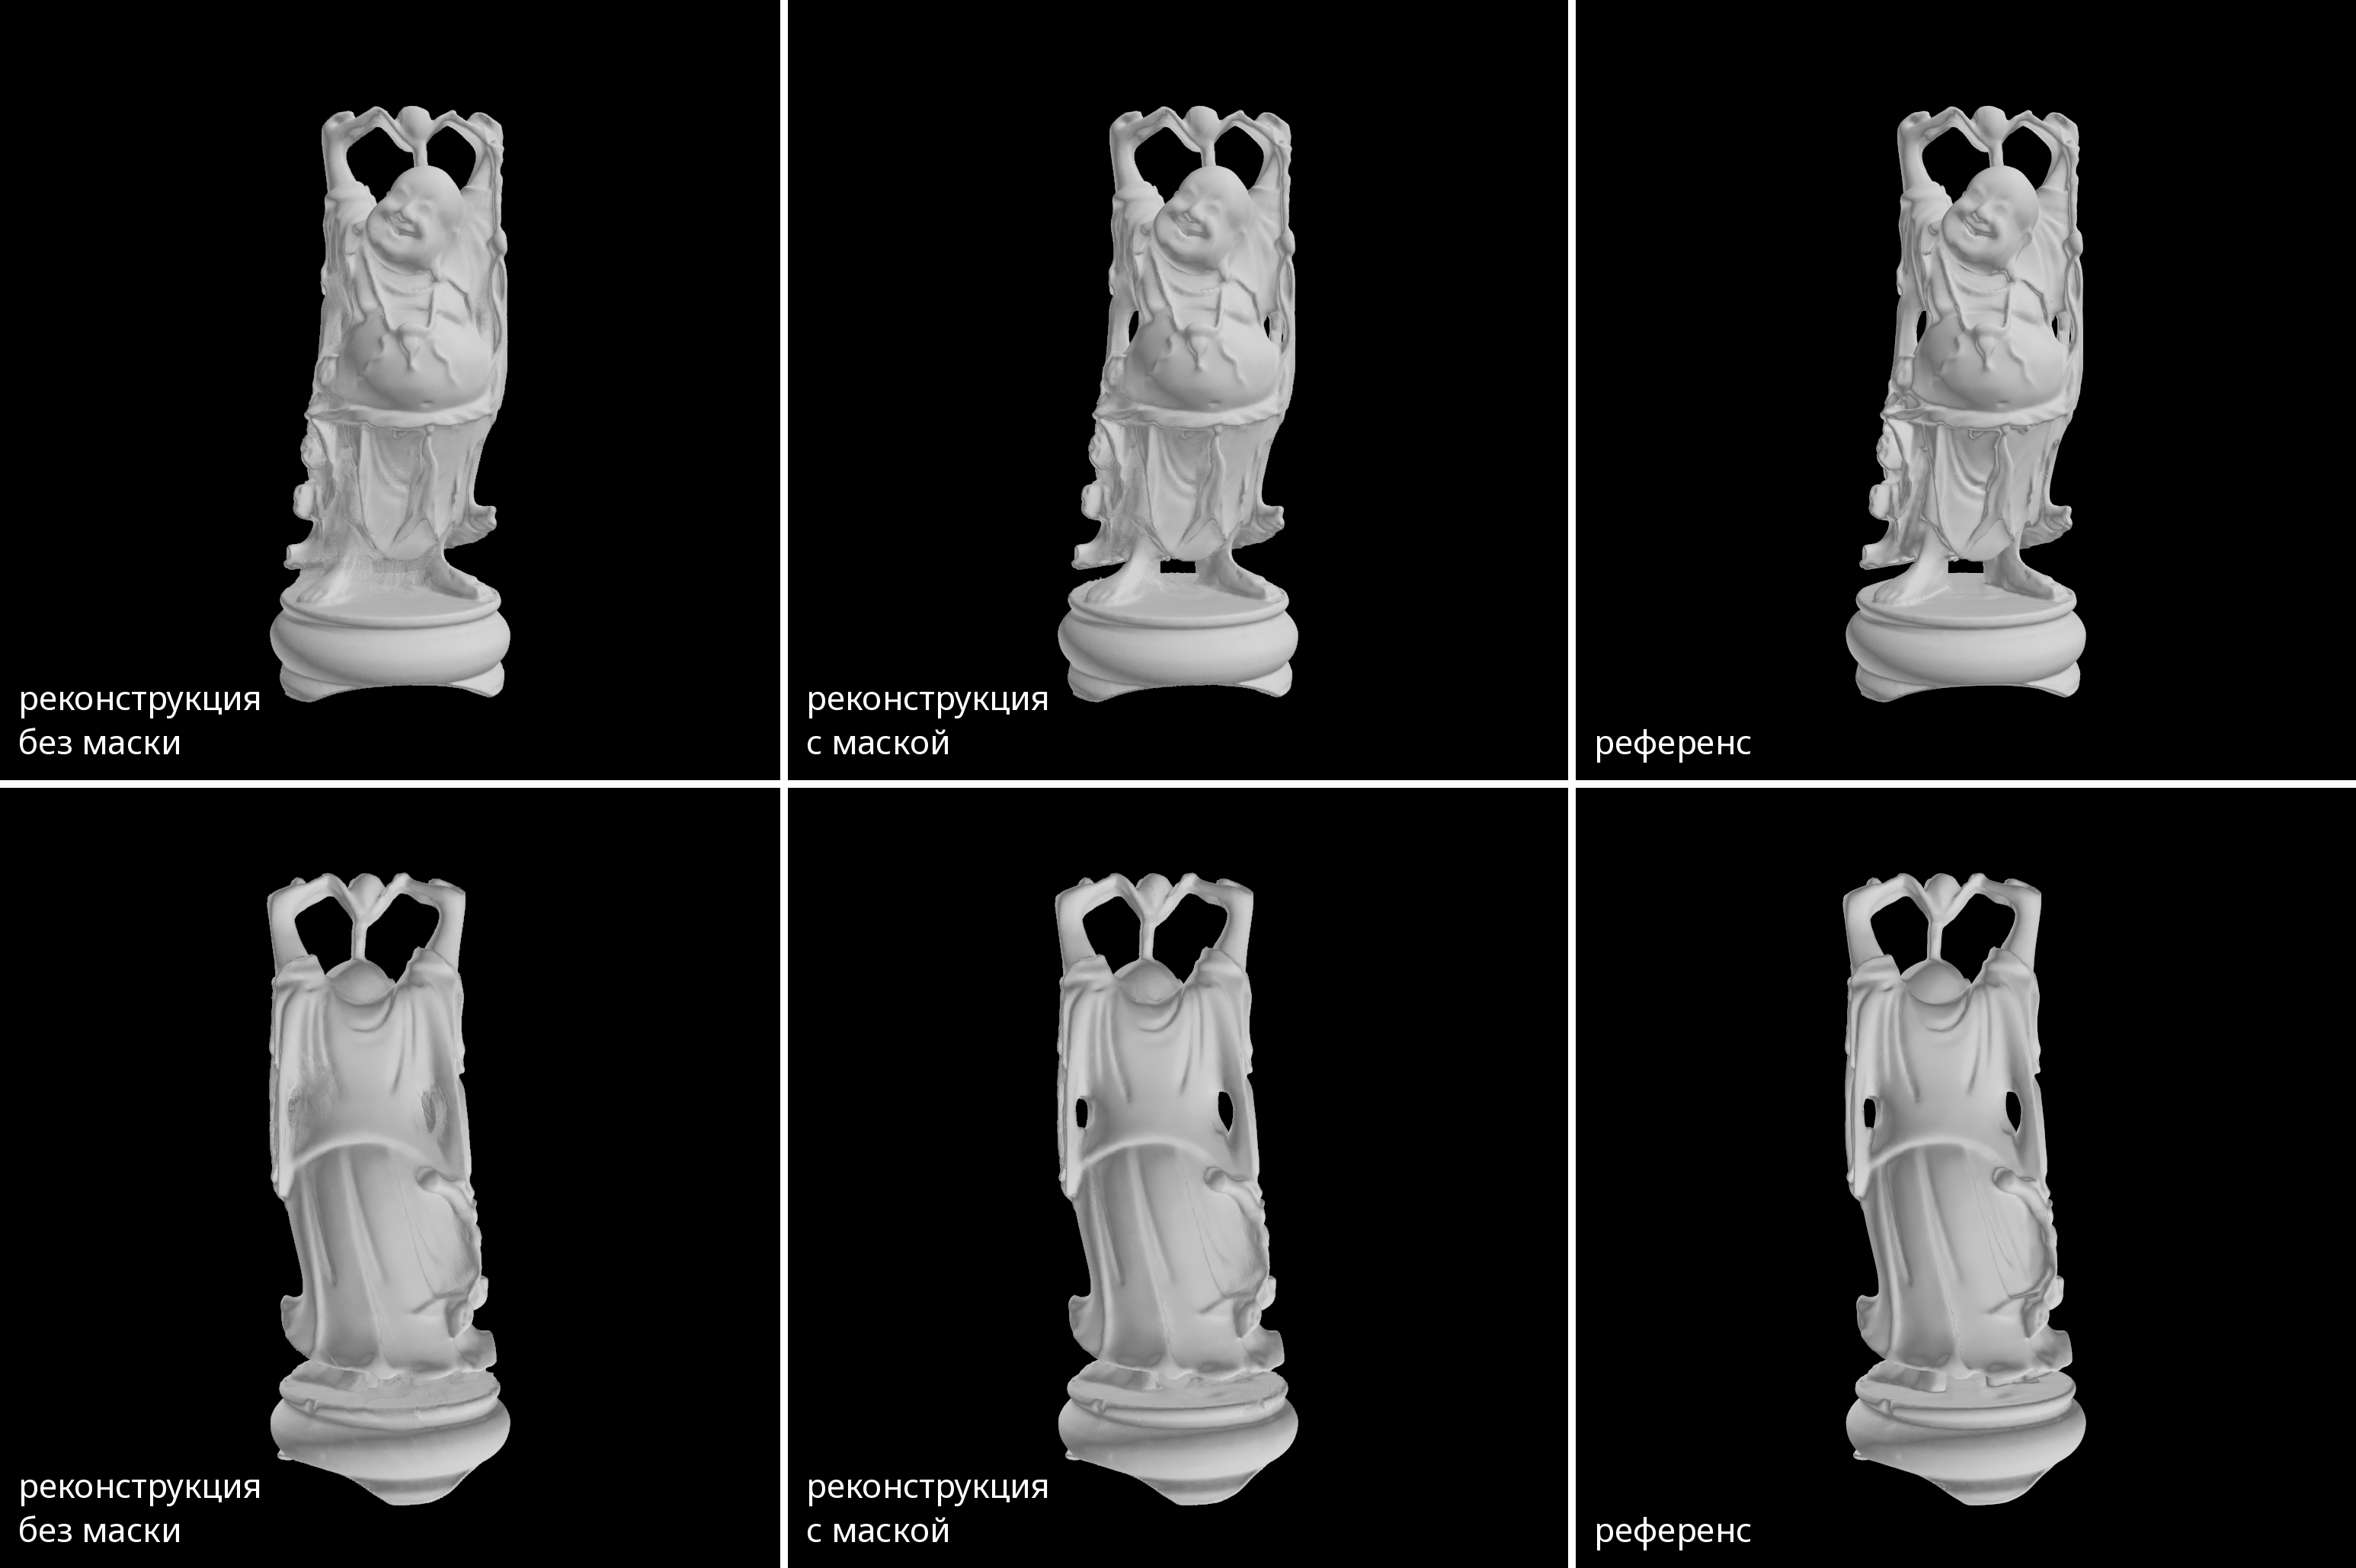
\includegraphics[width=0.9\textwidth]{collage_mask.png}
    \caption{Использование маски в процессе реконструкции. Слева -- результаты без использования маски. В центре -- результаты с маской. Справа -- референсные изображения.}
    \label{figAblMask}
\end{figure}

% 5. Использование sparsification в течение эпохи -- помогает с мелкими деталями -> Helicopter (примеры реконструкции с/без).
Во-вторых, в течение эпохи можно с определённым промежутком проводить этап разреживания модели, который по умолчанию применяется только между эпохами. В течение этого шага удаляются и добавляются брики в зависимости от их близости к поверхности, что позволяет "наращивать" представляемую область там, где происходит существенное добавление поверхности. На Рис. \ref{figAblSparsify} показаны примеры реконструкции без дополнительного разреживания и с ним, а также референсное изображение для наглядности. В первом случае винт вертолёта не смог восстановиться, так как он тонкий, поэтому на ранних эпохах его грубая версия не восстановилась, и брики, которые должны представлять его область пространства, были удалены. С дополнительным разреживанием на поздней эпохе эти брики, а следом и сам винт, были восстановлены.

\begin{figure}[t]
    \centering
    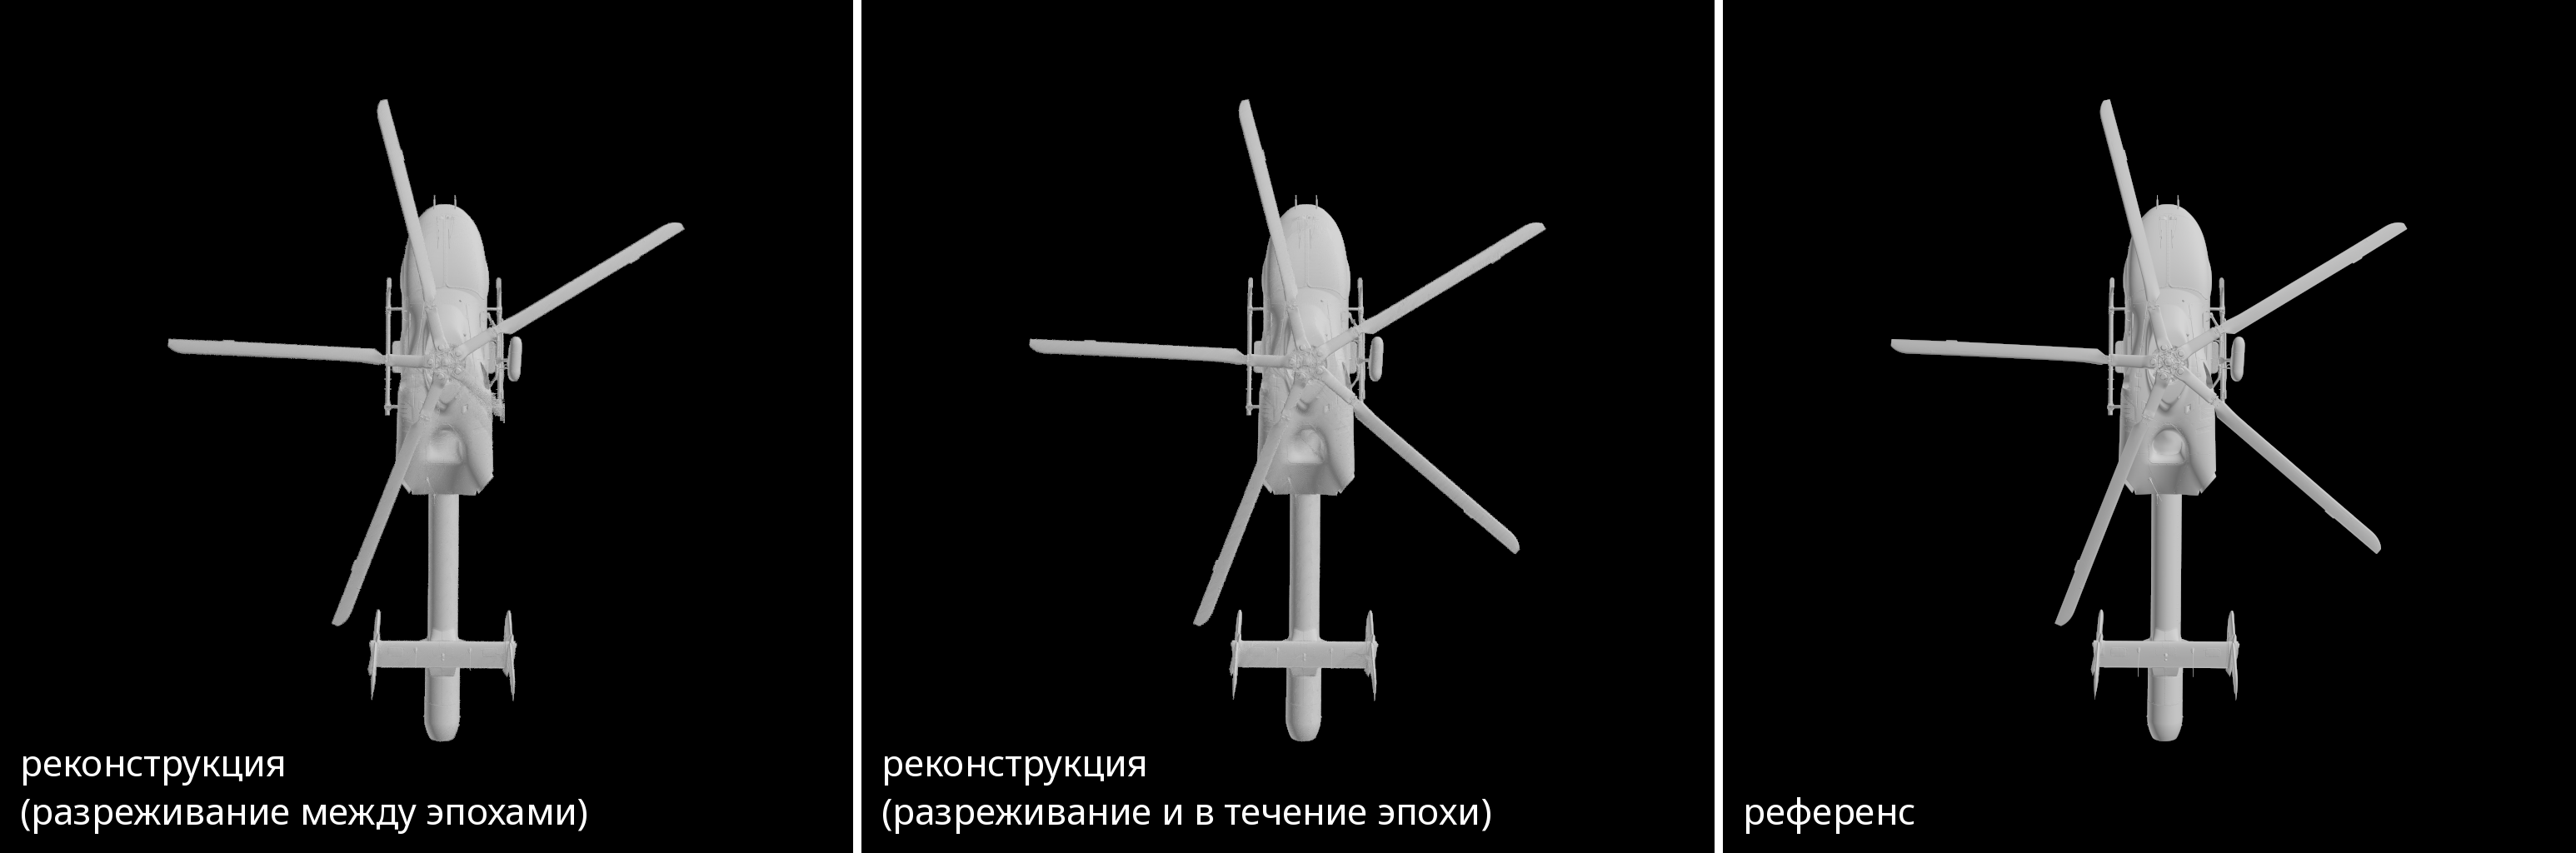
\includegraphics[width=0.9\textwidth]{collage_sparsify.png}
    \caption{Применение этапа разреживания/добавления бриков в течение эпохи. Слева -- результат с разреживанием только между эпохами. В центре -- результат с дополнительным разреживанием в течение эпох. Справа -- референсное изображение.}
    \label{figAblSparsify}
\end{figure}

% 6. Дополнительно: примеры реконструкции, разница в рендерах (синий-красный), среднее время работы на всех моделях.

На Рис. \ref{figExample1} показаны примеры реконструкции на моделях первой половины датасета. Они имеют относительно простую структуру, и изначально использовались для проверки работоспособности метода.

\begin{figure}[h]
    \centering
    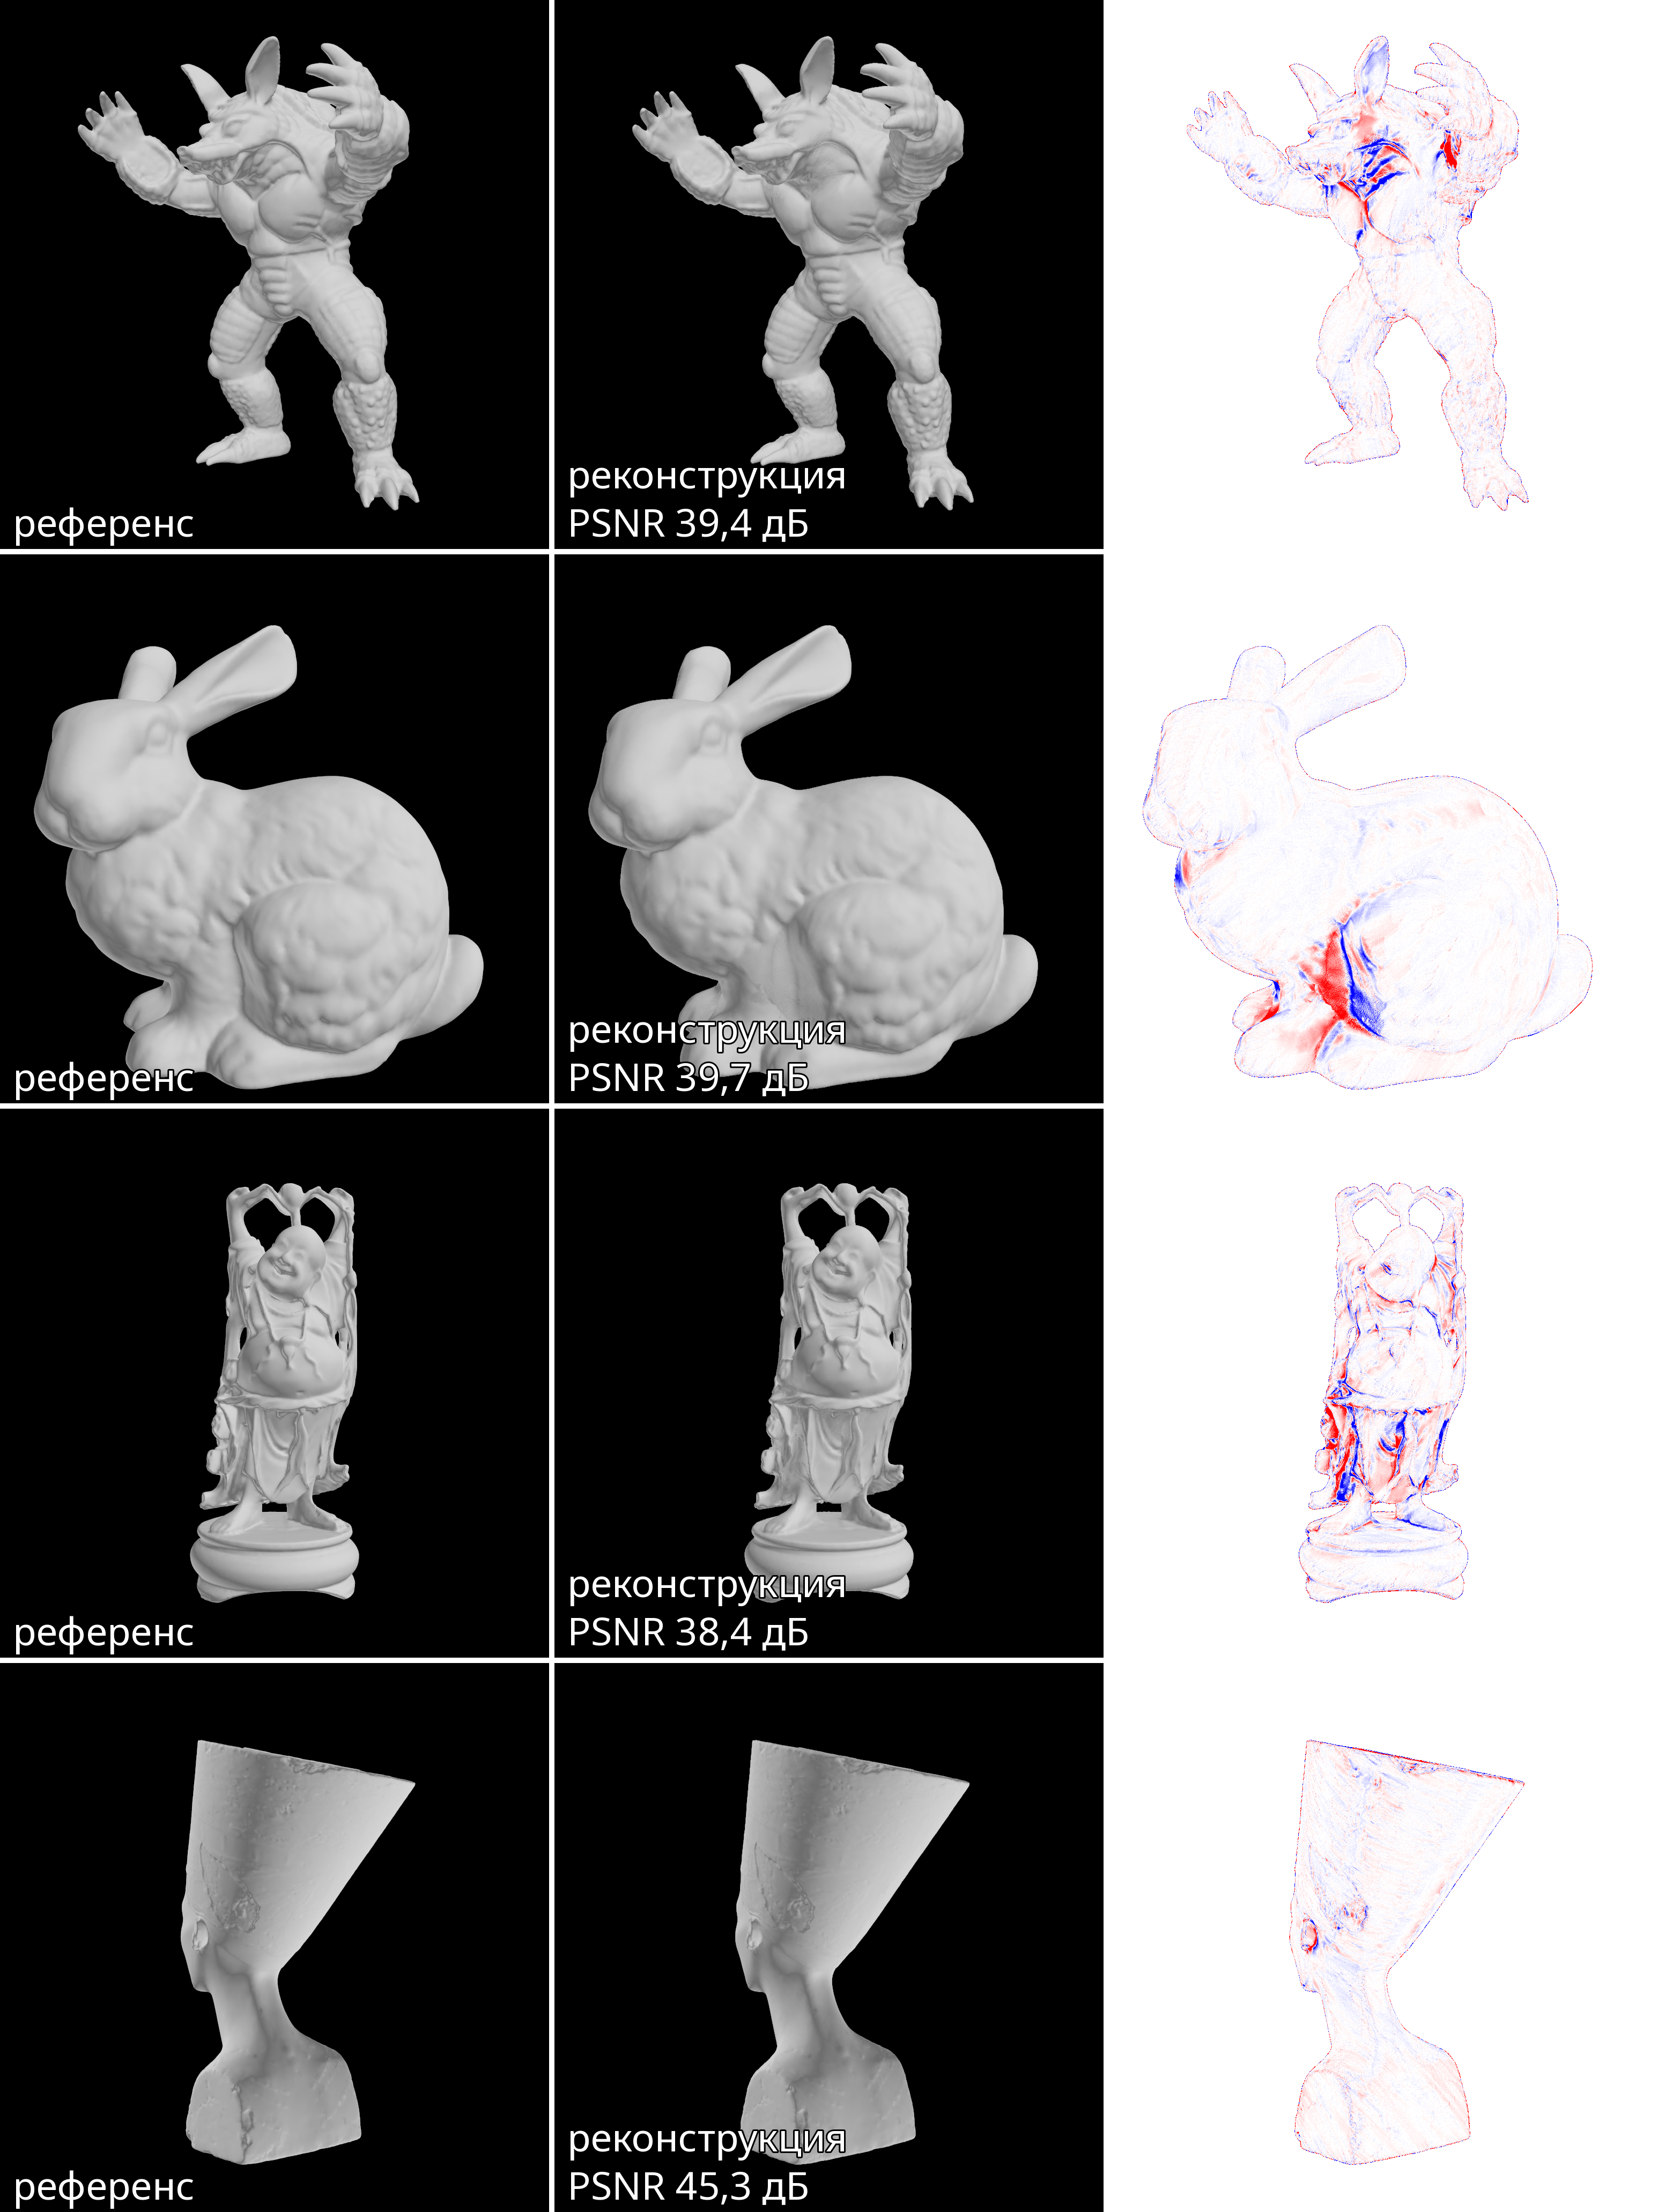
\includegraphics[width=0.9\textwidth]{collage1.png}
    \caption{Примеры реконструкции на моделях первой части датасета. Слева -- референс, в центре -- реконструкция, справа -- разница между рендерами, контраст увеличен для лучшей видимости.\label{figExample1}}
\end{figure}

На Рис. \ref{figExample2} показаны примеры реконструкции на моделях второй половины датасета. Эти модели отличаются высокой рельефностью поверхностей и наличием большого числа мелких деталей, поэтому отсутствие вторичных лучей (в обоих методах) сказывается на точности их реконструкции.

\begin{figure}[h]
    \centering
    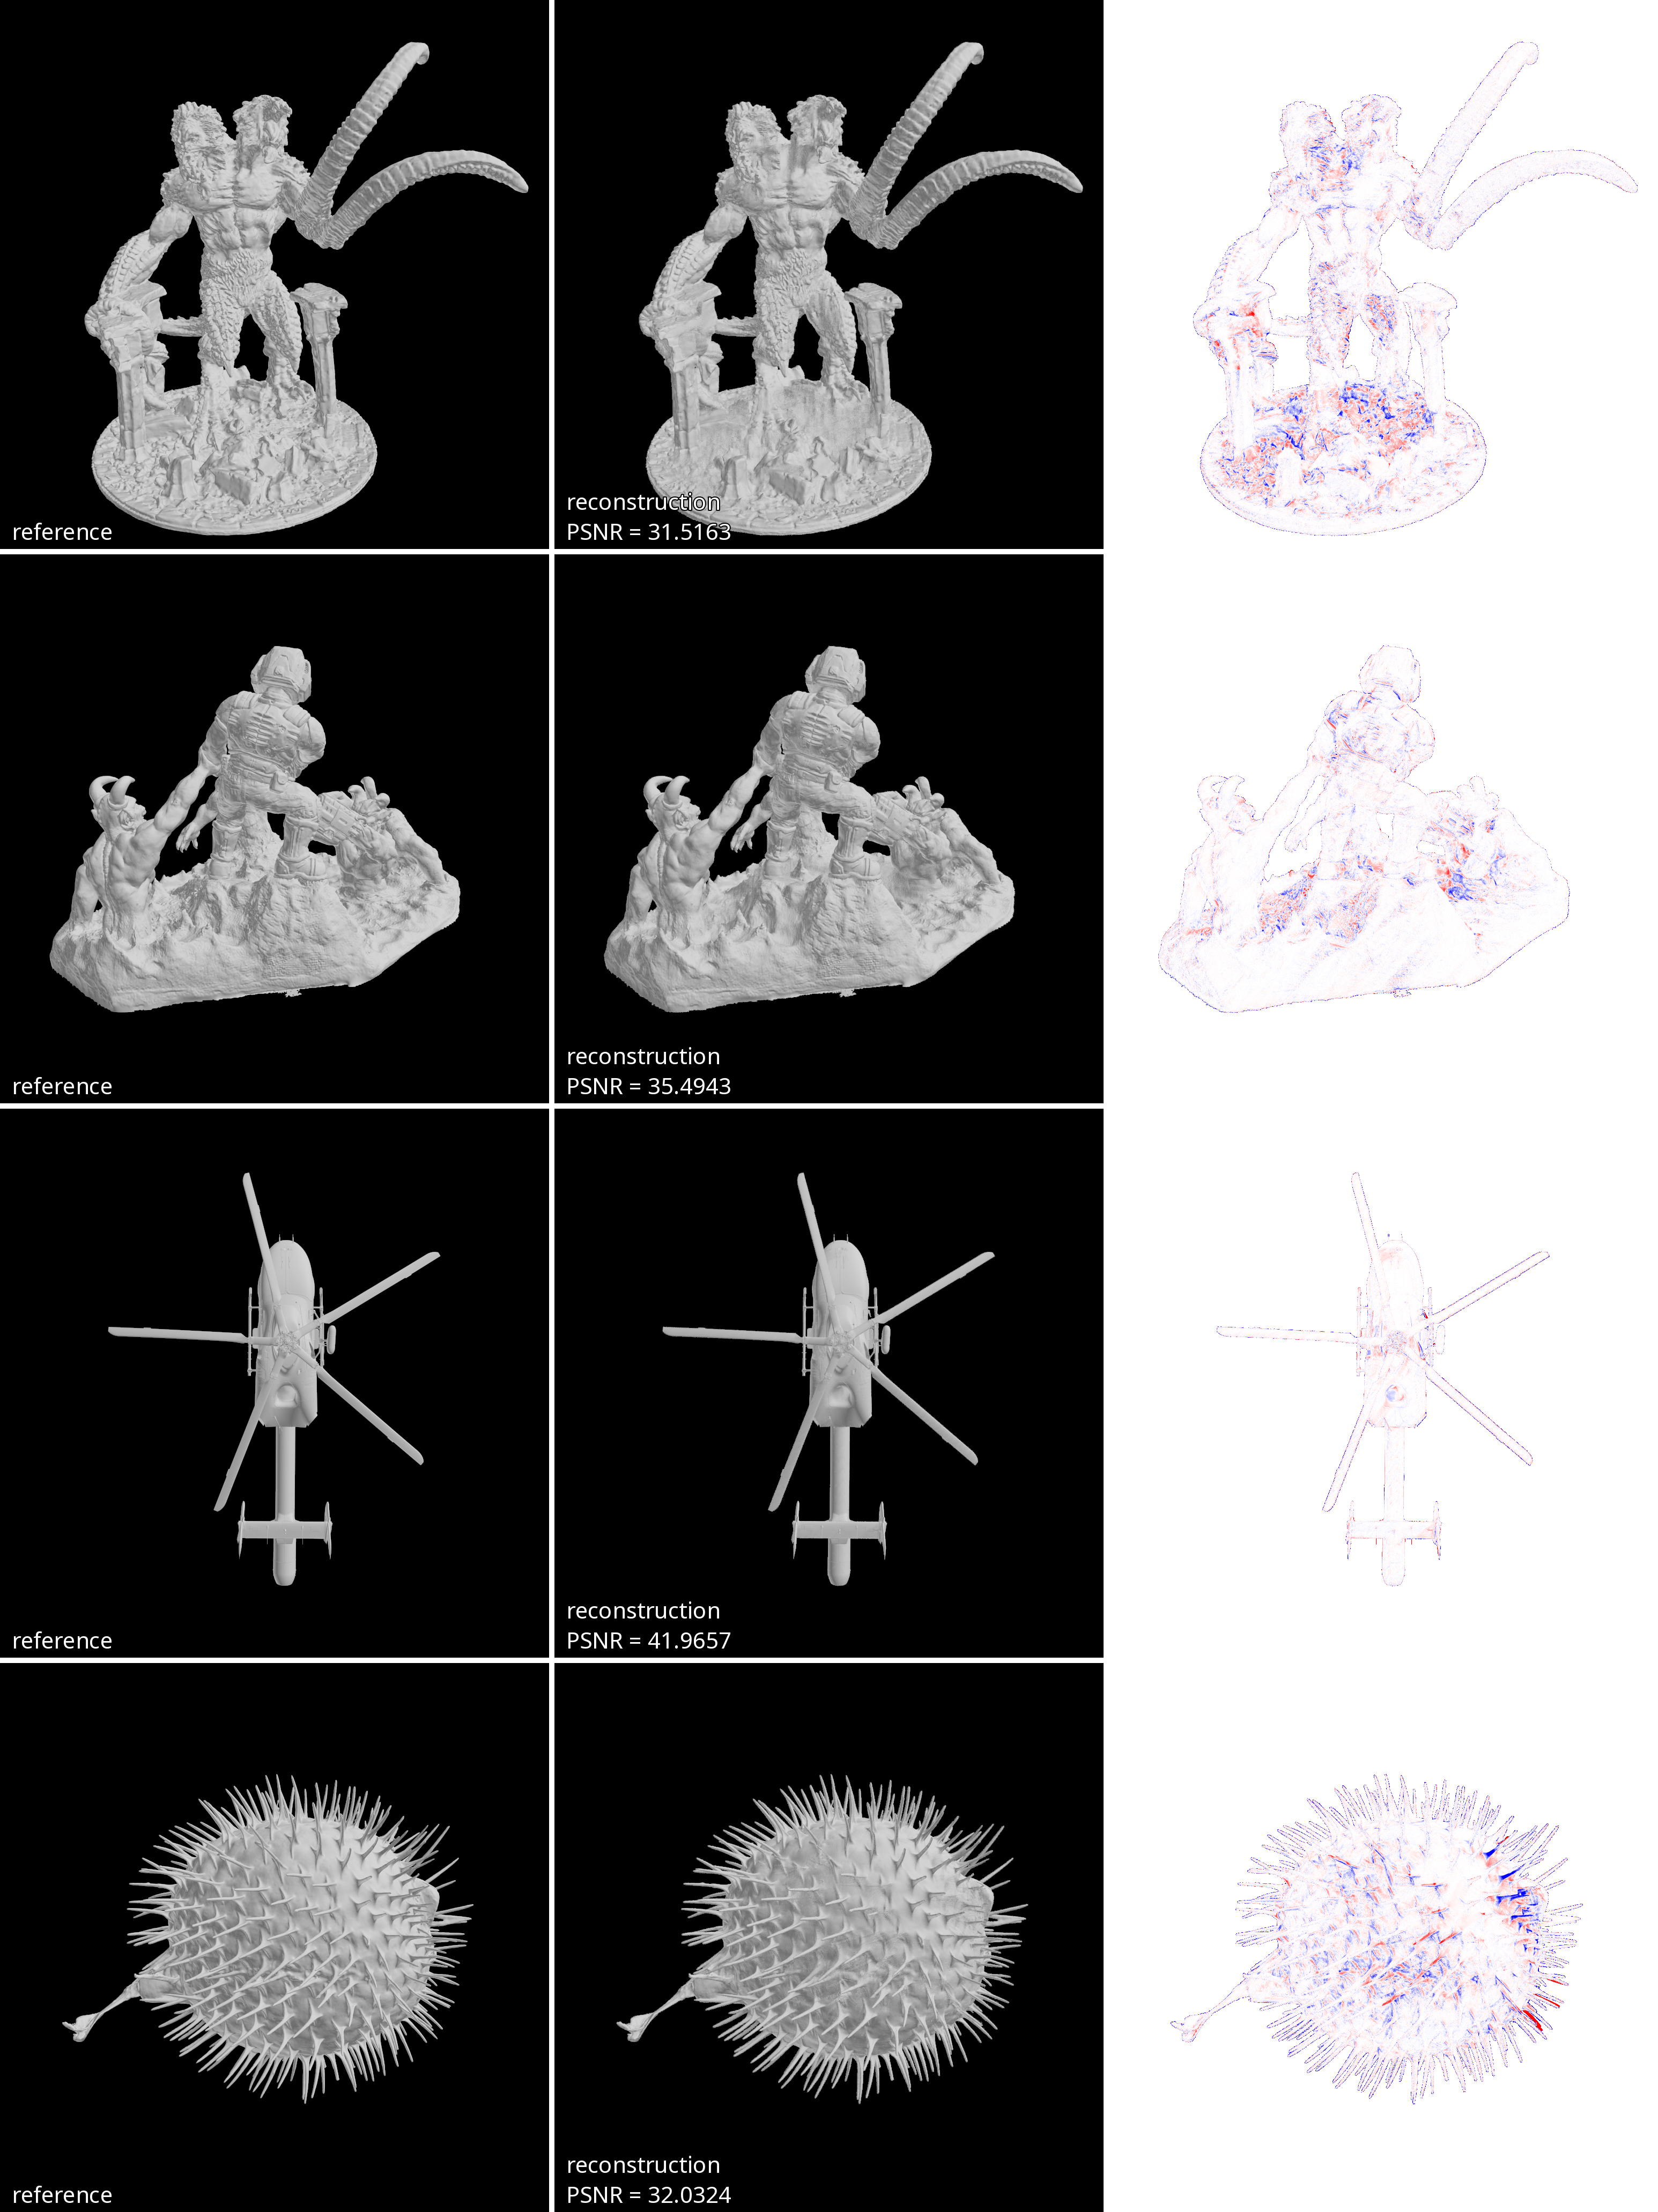
\includegraphics[width=0.9\textwidth]{collage2.png}
    \caption{Примеры реконструкции на моделях второй части датасета. Слева -- референс, в центре -- реконструкция, справа -- разница между рендерами, контраст увеличен для лучшей видимости.\label{figExample2}}
\end{figure}

% \begin{figure}[h]
%     \centering
%     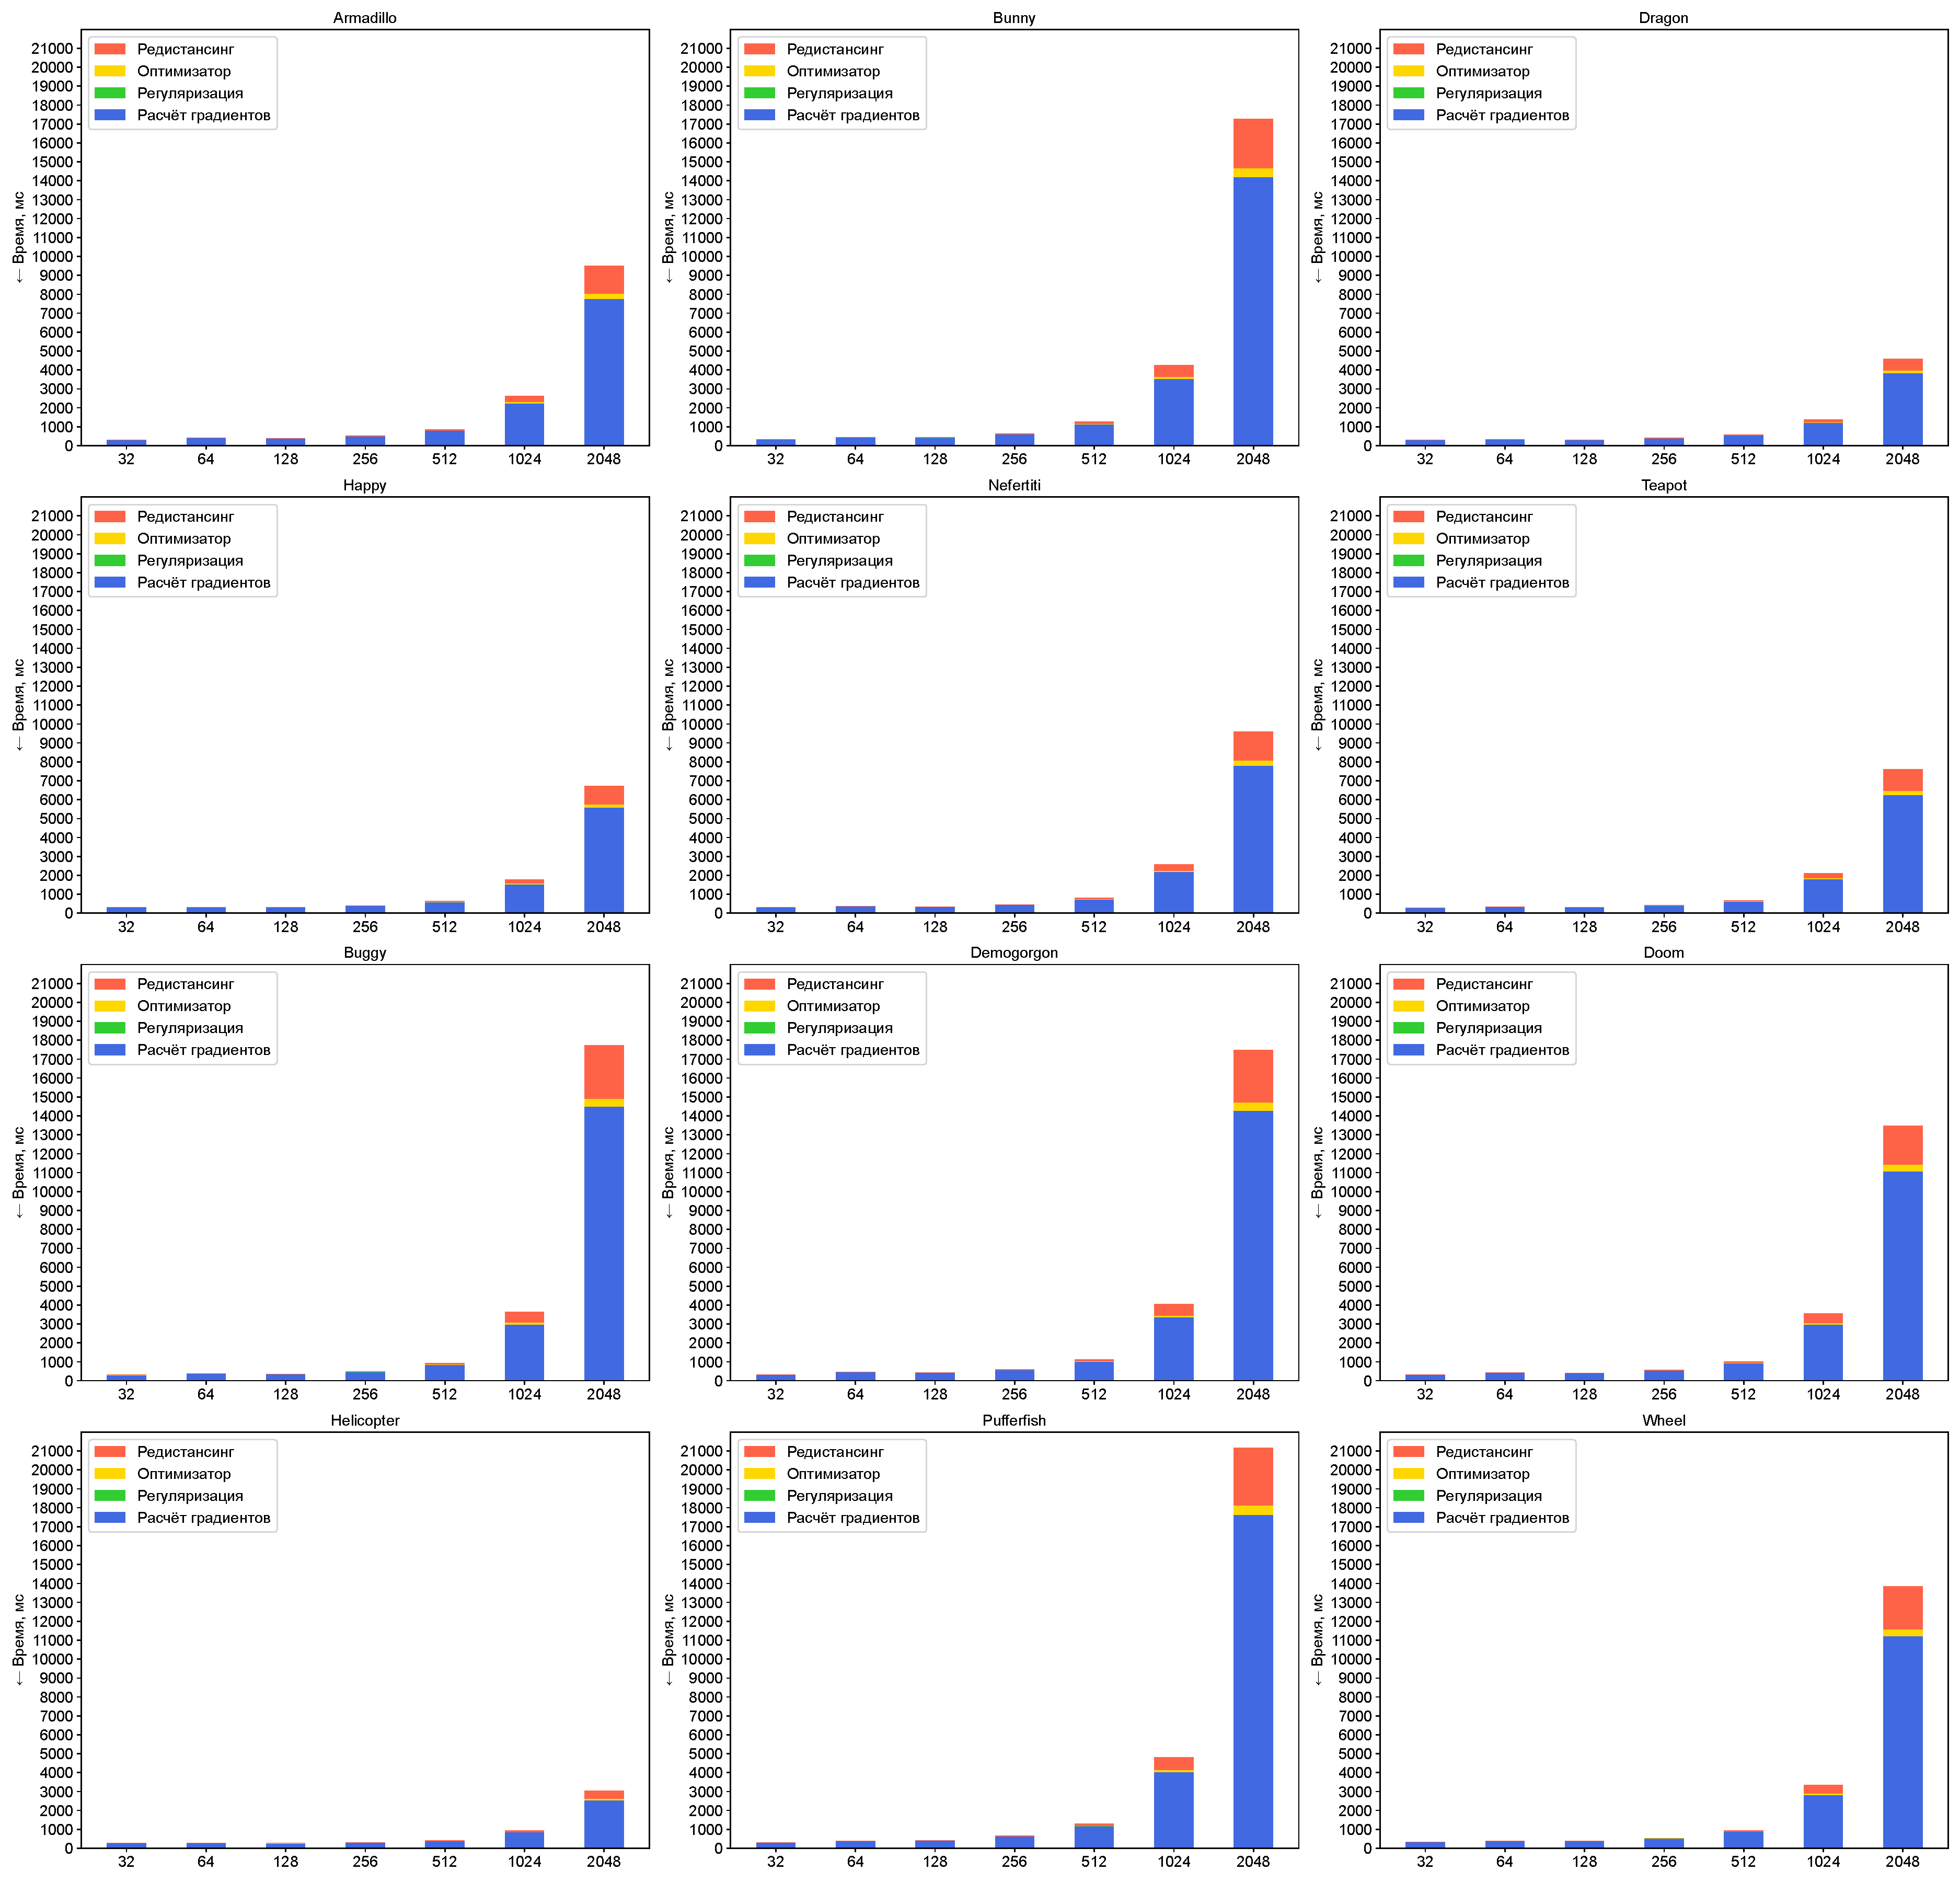
\includegraphics[width=0.95\textwidth]{ieee_acc_time_avg_big.pdf}
%     \caption{Среднее время рендеринга за одну эпоху для каждой модели. \label{figTimeBig}}
% \end{figure} 


\endinput